A neural network is a deep learning technique. Deep learning is a branch of machine learning and is from a mathematical perspective - A method of representing differential functions mapping one type of variable $x$, into another type of variable $y$.

$$
f(x) = y
$$

\noindent
Neural networks have high performance in detection and recognizing tasks. Through learning and classifying complex patterns and features, they can learn some representation of a given input. The neural network model is inspired by how biological neurons work in the brain. The objective of neural network models is to create a model that is teachable and can perform problem-solving tasks, which is easy for a human, but difficult for a computer.\\

\noindent
As for the brain, a neural network has neurons. These neurons are called nodes. These neurons are clustered in different layers, and each layer of neurons is in some way connected with other neurons in the other layers. A simple version of a neural network is the feed-forward neural network. In this kind of neural network, the connections are structured in a way such that there are no cycles in the graph. This implies the data travels only in one direction. This kind of architecture is composed of an input layer, one or more hidden layers, and an output layer. Given any kind of input variable X, the model creates its estimate of the output\_variable Y, after the input has been processed by the different layers.
In general, if you feed a model $\mathbb{K}$ the input variable $\mathbb{X}$, it will produce the output value $\mathbb{Y}:$

$$
\mathbb{K}: \mathbb{X} \to \mathbb{Y}
$$

\begin{figure}[!ht]
  \centering
  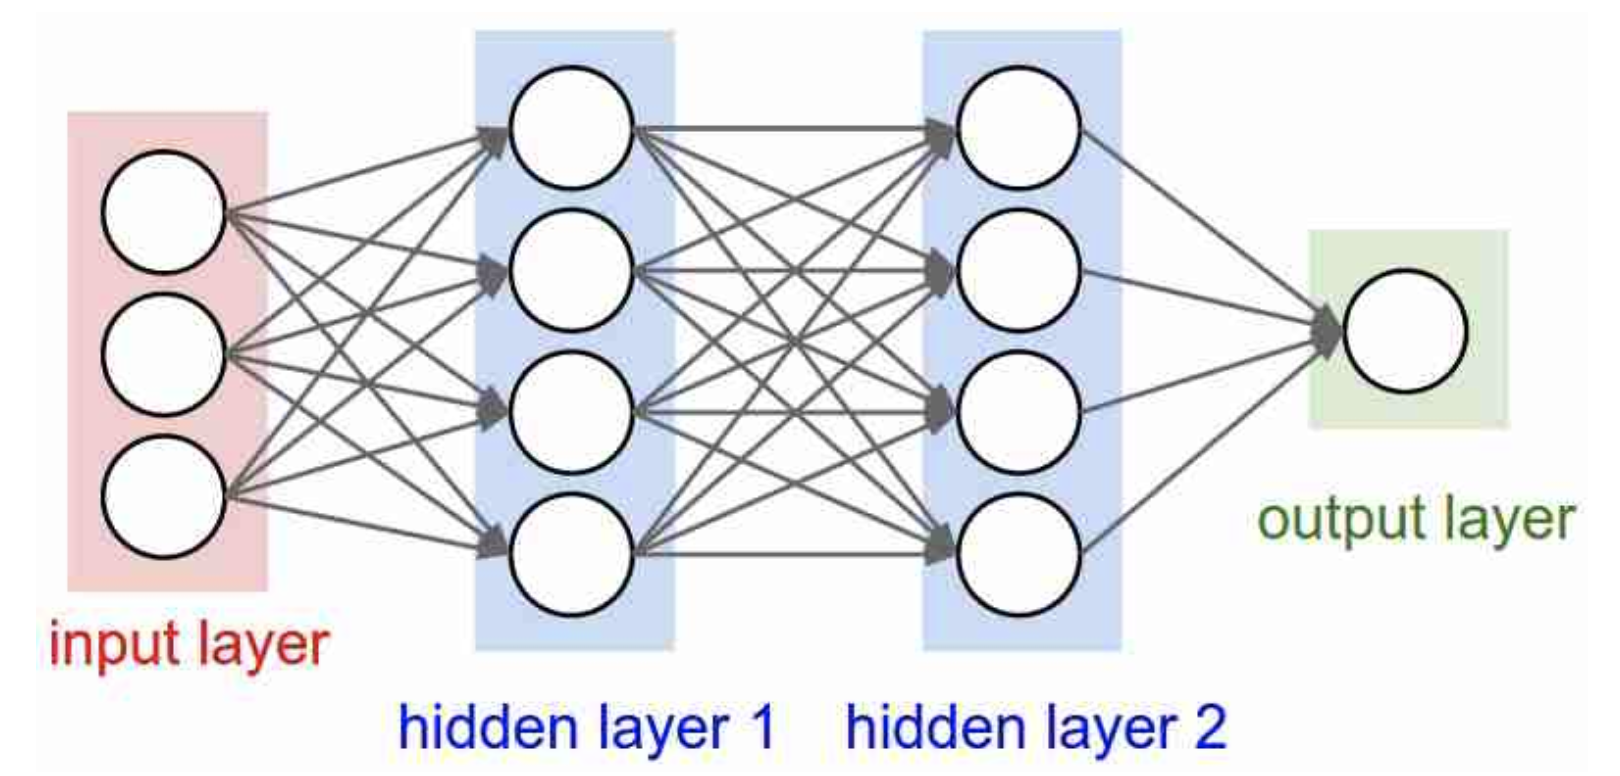
\includegraphics[scale=0.4]{latex/imgs/NN.png}
  \caption{Feed forward model, with two hidden layers.}\label{Baseline:before}
\end{figure}

\noindent
In our project we use two different types of neural networks, A convolutional neural network and recurrent neural network. These will be explained more in-depth later in the report.

\noindent
In machine learning, we have two methods of learning; supervised and unsupervised. Supervised learning is that for each input $\mathbb{X}$, the data also contains a target output $\mathbb{Y}$. The goal is to use some input to predict one or more given labeled outputs. Making the model learn an unknown function, which can map the input to the labeled output. Unsupervised learning does not have a corresponding target $\mathbb{Y}$ output for any part of the data. The goal is to learn some useful insight into the data's characteristics, without having a supervising label. In our project, we focused mainly on unsupervised learning, given we had limited labeled data, but a great amount of unlabeled data. \\
